\documentclass{article}
\usepackage{geometry}
\usepackage{titling}
\usepackage{hyperref}
\usepackage{amsmath}
\usepackage{amssymb}
\usepackage{graphicx}
\usepackage{caption}
\usepackage{subcaption}
\usepackage[dvipsnames]{xcolor}

\geometry{
  a4paper,
  total = {170mm, 257mm},
  left = 20mm,
  top = 20mm,
}
\graphicspath{ {./images/} }

\title{Trabajo práctico N° 4}
\author{Emanuel Nicolás Herrador}
\date{Abril 2025}

\makeatletter
\def\@maketitle{%
  \newpage
  \null
  \vskip 1em%
  \begin{center}%
  \let \footnote \thanks
    {\LARGE \@title \par}%
    \vskip 1em%
    {\large \@date}%
  \end{center}%
  \par
  \vskip 1em}
\makeatother

\begin{document}

\maketitle

\noindent\begin{tabular}{@{}ll}
	Estudiante & \theauthor \\
\end{tabular}

\section*{Ejercicio 2}
Veamos cada una por separado.
Comencemos con $\square\square\varphi \to \square\varphi$.
Notemos que por definición tenemos lo siguiente:
\begin{equation*}
	\begin{aligned}
		\sigma \vDash \square\square\varphi & \iff \forall j \geq 0 : \sigma[j..] \vDash \square\varphi                      \\
		                                    & \iff \forall j \geq 0 : \forall j_2 \geq 0 : \sigma[j..][j_2..] \vDash \varphi \\
		                                    & \iff \forall i \geq 0 : \sigma[i..] \vDash \varphi                             \\
		                                    & \iff \sigma \vDash \square\varphi
	\end{aligned}
\end{equation*}
Luego, es trivial que se verifica la implicación porque son fórmulas equivalentes.

Para $\square(\varphi \land \psi) \to \square\varphi \land \square\psi$ veamos que:
\begin{equation*}
	\begin{aligned}
		\sigma \vDash \square(\varphi \land \psi) & \iff \forall j \geq 0 : \sigma[j..] \vDash \varphi \land \psi                                               \\
		                                          & \iff \forall j \geq 0 : \sigma[j..] \vDash \varphi \land \sigma[j..] \vDash \psi                            \\
		                                          & \iff (\forall j \geq 0 : \sigma[j..] \vDash \varphi) \land (\forall j_2 \geq 0 : \sigma[j_2..] \vDash \psi) \\
		                                          & \iff \sigma \vDash \square\varphi \land \sigma \vDash \square\psi                                           \\
		                                          & \iff \sigma \vDash \square\varphi \land \square\psi
	\end{aligned}
\end{equation*}
Con ello, resulta trivial la implicación al ser fórmulas equivalentes.

Y, por último, queda ver que $\diamondsuit(\varphi \lor \psi) \to \diamondsuit\varphi \lor \diamondsuit\psi$:
\begin{equation*}
	\begin{aligned}
		\sigma \vDash \diamondsuit(\varphi \lor \psi) & \iff \exists j \geq 0 : \sigma[j..] \vDash (\varphi \lor \psi)                                             \\
		                                              & \iff \exists j \geq 0 : \sigma[j..] \vDash \varphi \lor \sigma[j..] \vDash \psi                            \\
		                                              & \iff (\exists j \geq 0 : \sigma[j..] \vDash \varphi) \lor (\exists j_2 \geq 0 : \sigma[j_2..] \vDash \psi) \\
		                                              & \iff \sigma \vDash \diamondsuit\varphi \lor \sigma \vDash \diamondsuit\psi                                 \\
		                                              & \iff \sigma \vDash (\diamondsuit\varphi \lor \diamondsuit\psi)
	\end{aligned}
\end{equation*}
Luego, al ser equivalentes, claramente se cumple la implicación.

\section*{Ejercicio 3}
Ver la validez de la fórmula equivale a ver si se cumple la equivalencia dada por $\square(p \land \diamondsuit q) \equiv \square(p \text{U} q)$.
Para ello, una forma de refutar la validez es mostrar una traza que cumple una propiedad pero la otra no.
Veamos que $(\{q\})^\omega$ cumple claramente $\square(p \text{U} q)$ pero no $\square(p \land \diamondsuit q)$.
Luego, se refuta. $\blacksquare$

\section*{Ejercicio 4}
Se pretende demostrar formalmente que \textit{strong fairness} implica \textit{weak fairness}.
Es decir, es quiere ver que $(\square\diamondsuit\varphi \to \square\diamondsuit \psi) \to (\diamondsuit\square\varphi \to \square\diamondsuit\psi)$.

Para ello, expandamos cada una de las partes:
\begin{equation*}
	\begin{aligned}
		\square\diamondsuit\varphi \to \square\diamondsuit\psi & \equiv \neg\square\diamondsuit\varphi \lor \square\diamondsuit\psi \\
		\diamondsuit\square\varphi \to \square\diamondsuit\psi & \equiv \neg\diamondsuit\square\varphi \lor \square\diamondsuit\psi
	\end{aligned}
\end{equation*}

Ahora, supongamos que \textit{strong fairness} vale para un $\sigma$ dado que $\sigma \vDash \square\diamondsuit\psi$.
Luego, es claro que, por la anterior expansión, también vale \textit{weak fairness} para $\sigma$.

En caso de que valiera \textit{strong fairness} pero solo porque $\sigma \vDash \neg\square\diamondsuit\varphi$, podemos notar lo siguiente:
\begin{equation}
	\tag*{(4.1)}
	\begin{aligned}
		\sigma \vDash \neg\square\diamondsuit\varphi & \iff \neg(\forall i \geq 0 : \exists j \geq 0 : \sigma[i..][j..] \vDash \varphi) \\
		                                             & \iff \exists i \geq 0 : \forall j \geq 0 : \sigma[i..][j..] \vDash \neg\varphi   \\
		                                             & \iff \exists i \geq 0 : \forall j \geq i : \sigma[j..] \vDash \neg\varphi        \\
	\end{aligned}
\end{equation}

Ahora, nuestro objetivo es llegar a $\sigma \vDash \neg\diamondsuit\square\varphi$, lo cual significa que:
\begin{equation}
	\tag*{(4.2)}
	\begin{aligned}
		\sigma \vDash \neg\diamondsuit\square\varphi & \iff \neg(\exists i \geq 0 : \forall j \geq 0 : \sigma[i..][j..] \vDash \neg\varphi) \\
		                                             & \iff \forall i \geq 0 : \exists j \geq 0 : \sigma[i..][j..] \vDash \neg\varphi       \\
		                                             & \iff \forall i \geq 0 : \exists j \geq i : \sigma[j..] \vDash \neg\varphi
	\end{aligned}
\end{equation}

Si $\sigma \vDash \neg\square\diamondsuit\varphi$, entonces por $(4.1)$ es de la forma $(\emptyset + \{\varphi\} + \{\psi\} + \{\varphi, \psi\})^*(\emptyset + \{\psi\})^\omega$.
Con ello, claramente $\sigma \vDash \neg\diamondsuit\square\varphi$ por $(4.2)$ porque sea $j$ el índice más chico a partir del cual todo elemento de la traza cumple $\neg\varphi$, entonces $\forall 0 \leq i \leq j : \sigma[j..] \vDash \neg\varphi$ y $\forall j \leq i : \sigma[i..] \vDash \neg\varphi$.

Por esto, se demuestra por completo que \textit{strong fairness} implica \textit{weak fairness} dado que si una traza satisface la primera, entonces también satisfará la segunda. $\blacksquare$

\section*{Ejercicio 5}
Veamos cada una:
\begin{itemize}
	\item ``Si $\varphi$ es cierto durante la ejecución del programa, eventualmente ocurrirá $\psi$'': $\square(\varphi \to \diamondsuit\psi)$.
	\item ``No es posible que $\varphi$ y $\psi$ ocurran simultáneamente durante la ejecución del programa'': $\neg\diamondsuit(\varphi \land \psi)$.
	\item ``Cada vez que $\varphi$ sea cierto, $\psi$ también lo es'': $\square(\varphi \to \psi)$.
	\item ``$\varphi$ no deja de ocurrir, al menos hasta que $\psi$ ocurra'': $\varphi \text{WU} \psi \equiv \square\varphi \lor (\varphi \text{U} \psi)$.
\end{itemize}

\section*{Ejercicio 6}
Se define el operador \textit{while} como:
\begin{equation*}
	\tag*{(6.1)}
	\sigma \vDash \varphi \text{W} \psi \iff \forall i \geq 0 : (\forall 0 \leq j \leq i : \sigma[j..] \vDash \psi) \Rightarrow \sigma[i..] \vDash \varphi
\end{equation*}

Para poder resolver los siguientes items de este ejercicio, va a ser útil desglosar la definición para entenderla a detalle.
Tomemos la definición de $(6.1)$ y digamos que tenemos el mayor $x$ tal que $\forall 0 \leq j \leq x : \sigma[j..] \vDash \psi$.
Ahora, por la definición, sabemos que $\sigma[x..] \vDash \varphi$.
Además, es trivial notar que $\forall 0 \leq j \leq x-1 : \sigma[j..] \vDash \psi$, por lo que por definición $\sigma[(x-1)..] \vDash \varphi$.
Expandiendo esta idea, llegamos a que $\forall 0 \leq j \leq x : \sigma[j..] \vDash \psi$.

Con lo anterior, la definición puede pasar a ser:
\begin{equation*}
	\tag*{(6.2)}
	\sigma \vDash \varphi \text{W} \psi \iff \forall i \geq 0 : (\forall 0 \leq j \leq i : \sigma[j..] \vDash \psi) \Rightarrow (\forall 0 \leq j \leq i : \sigma[j..] \vDash \varphi)
\end{equation*}

El \textbf{primer punto} solicita expresar el operador \textit{while} en términos del \textit{until} y expresiones booleanas.
Para ello, podremos pensar que siempre en el prefijo se cumple $\psi \to \varphi$ hasta que deja de cumplirse $\psi$.
Es decir: $\varphi \text{W} \psi \equiv ((\psi \to \varphi) \text{U} \neg\psi) \lor \square(\psi \land \varphi)$.

Finalmente, el \textbf{segundo punto} pide expresar el operator \textit{until} en términos del \textit{while} y operaciones booleanas.
Aquí, como queremos que el until sea $\varphi \text{U} \psi$ y dada la definición vista anteriormente, tomaremos algo de la forma $\gamma \text{W} \neg\psi \land \diamondsuit\psi$.
De este modo, tendremos que $\gamma \text{W} \neg\psi \land \diamondsuit\psi \equiv (((\neg\psi \to \gamma) \text{U} \psi) \lor \square(\neg\psi \land \gamma)) \land \diamondsuit\psi$.
Como no puede cumplirse al mismo tiempo $\square(\neg\psi \land \gamma)$ y $\diamondsuit\psi$, tenemos que $\gamma \text{W} \neg\psi \land \diamondsuit\psi \equiv (\neg\psi \to \gamma) \text{U} \psi \land \diamondsuit\psi$.
Ahora, al ser un until, $\diamondsuit\psi$ resulta redundante dado que el until ya garantiza que en algún momento $\psi$ sucederá.
Por ello, podemos considerar $\gamma \text{W} \neg\psi \land \diamondsuit\psi \equiv (\neg\psi \to \gamma) \text{U} \psi$.
Finalmente, se busca que $\neg\psi \to \gamma \equiv \varphi$.
Si bien esto no es posible, podemos considerar $\gamma = \varphi$ tal que $\varphi \text{W} \neg\psi \land \diamondsuit\psi \equiv (\neg\psi \to \varphi) \text{U} \psi$.

Si bien este último punto es diferente al until que queremos, igualmente es válido dado que cuando valga por primera vez $\psi$ este marcará el final del until.
En las posiciones anteriores a este final, se cumplirá $\neg\psi$ por lo que el implica determina que vale $\varphi$ en cada paso anterior.
Por ello, finalmente, consideramos $\varphi \text{U} \psi \equiv \varphi \text{W} \neg\psi \land \diamondsuit\psi$

Notar que ninguno de los puntos se pudo satisfacer dado que se tuvieron que utilizar operadores temporales además del until y el while.

% TODO: Consultar al profesor.
\begin{quotation}
	\textbf{\textcolor{Red}{Nota:}} ¿Está bien justificarlo de este modo o debo expandir sí o sí con el para todo y existe?
\end{quotation}

\section*{Ejercicio 7}
Queremos definir el operador $\text{Z}$ tal que $\varphi \text{Z} \psi$ represente la propiedad de que siempre entre dos posiciones distintas en las cuales valga $\varphi$, existe una en la que vale $\psi$.
Considero que estar entre medio de las otras dos implica que no se consideran los extremos.

Motivo de ello, la definición que doy es la siguiente: $\square(\varphi \to \neg\bigcirc(\neg\psi \text{U} \varphi))$.
Es decir, me concentro en la negación de la propiedad para definirla.
Considero que cuando ``veo'' un $\varphi$, entonces a partir de la siguiente posición no puede pasar que veo otro $\varphi$ antes de algún $\psi$.

%TODO: Consultar al profesor 
\begin{quotation}
	\textbf{\textcolor{Red}{Nota:}} En ejercicios de este tipo, ¿basta con dar la definición y explicar la idea? ¿O cómo deberíamos justificarlo?
\end{quotation}

\section*{Ejercicio 8}
Veamos cada autómata con alfabeto $\{a, b, c\}$ por separado.

Para el caso de conjunto de cadenas infinitas con una cantidad finita de $a$ tenemos el siguiente diagrama:
\begin{figure}[!htb]
	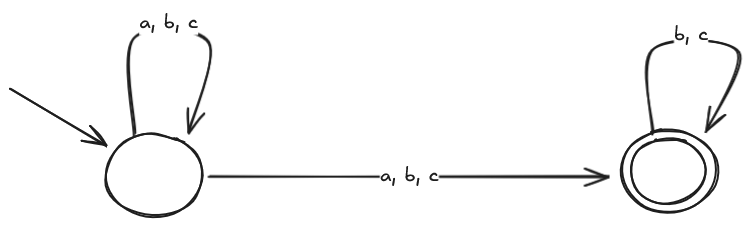
\includegraphics[width=0.7\textwidth]{04-08-a.png}
	\centering
\end{figure}

Para el conjunto de cadenas infinitas en que cada ocurrencia de $c$ viene inmediatamente seguida de una ocurrencia de $b$ tenemos:
\begin{figure}[!htb]
	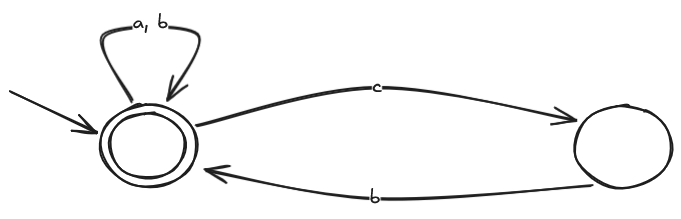
\includegraphics[width=0.7\textwidth]{04-08-b.png}
	\centering
\end{figure}

Para el conjunto de cadenas infinitas que no terminen en una secuencia infinita de $a$ ni en una de $b$ ni en una de $c$ tenemos:
\begin{figure}[!htb]
	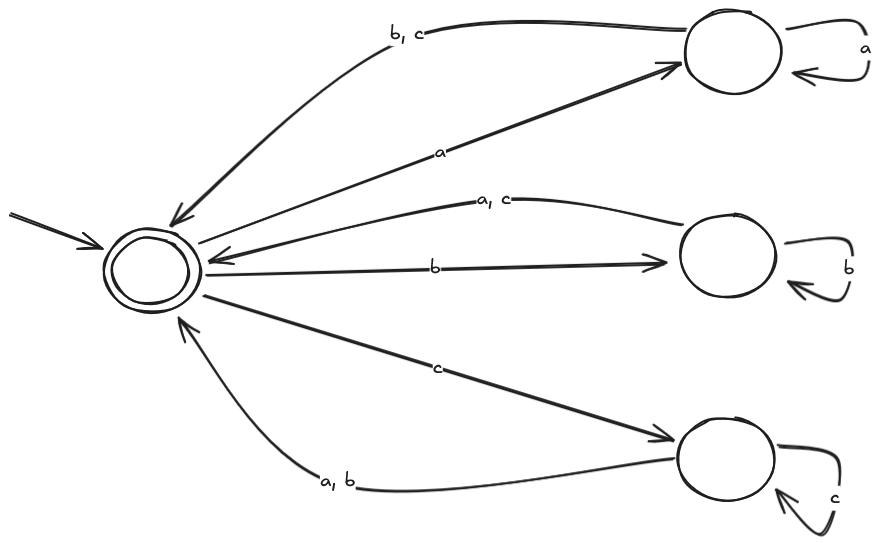
\includegraphics[width=0.7\textwidth]{04-08-c.png}
	\centering
\end{figure}

\pagebreak
Y para el conjunto de cadenas infinitas con cantidades finitas de $a$, $b$ y $c$, interpreto que se quiso referir a que alguna de las tres es finita porque si las tres lo son al mismo tiempo, la cadena no puede ser infinita.
Por ello, el diagrama nos queda:
\begin{figure}[!htb]
	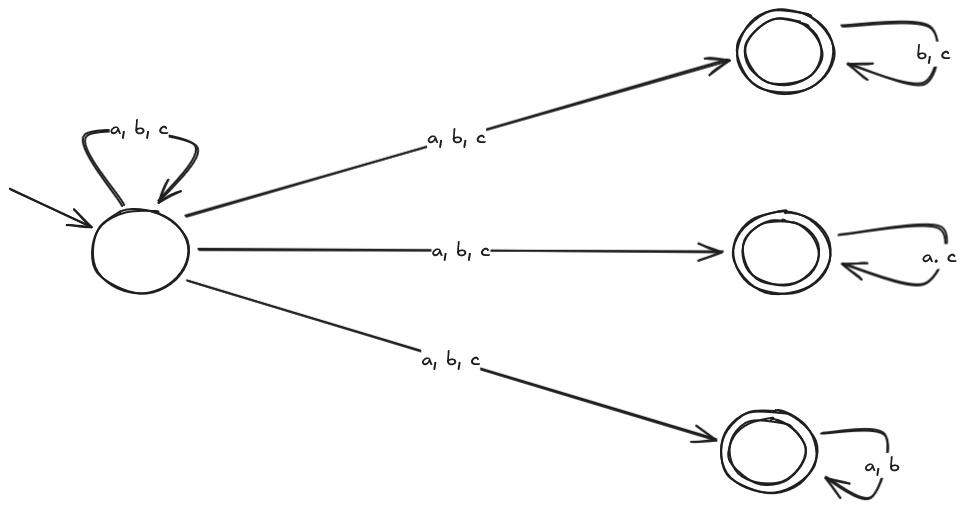
\includegraphics[width=0.7\textwidth]{04-08-d.png}
	\centering
\end{figure}

\begin{quotation}
	\textbf{\textcolor{Red}{Nota:}} ¿Es correcta la interpretación del último punto de este ejercicio?
\end{quotation}

\section*{Ejercicio 9}
Notemos que el diagrama de la izquierda representa el lenguaje $\omega$-regular $b^*a(a + b)^\omega$ mientras que el de la derecha a $(a + b)^*a(a + b)^\omega$.
Por ello, aceptan el mismo lenguaje $\omega$-regular porque el no determinismo de la transición $a$ en el autómata de la derecha se puede resolver tomando siempre la transición que conecta ambos estados.
Se puede verificar que esto no modifica el lenguaje del autómata porque en ambos estados puede tomar las mismas acciones, por lo que se sigue cumpliendo que toda traza con al menos una $a$ sea aceptada.

Respecto al lenguaje $\omega$-regular, como bien se dijo antes, es aquél que expresa que toda traza con al menos una $a$ es aceptada.
Por motivos de facilidad para notar el prefijo que se quiere, considero la expresión no determinística del autómata de la derecha.

\begin{quotation}
	\textbf{\textcolor{Red}{Nota:}} ¿Es correcto o cómo debemos solucionar un ejercicio de este estilo?
\end{quotation}

\pagebreak
\section*{Ejercicio 10}
Las expresiones $\omega$-regulares tratadas en los ejercicios 8, 9 y 10 de la anterior guía se presentan a continuación junto con el autómata de Büchi correspondiente:
\begin{figure}[!htb]
	\renewcommand\thesubfigure{\arabic{subfigure}}
	\centering
	\begin{subfigure}[b]{0.2\textwidth}
		\centering
		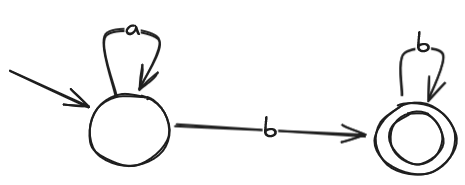
\includegraphics[width=\textwidth]{04-10-01.png}
		\caption{$a^*b^\omega$}
	\end{subfigure}
	\hfil
	\begin{subfigure}[b]{0.3\textwidth}
		\centering
		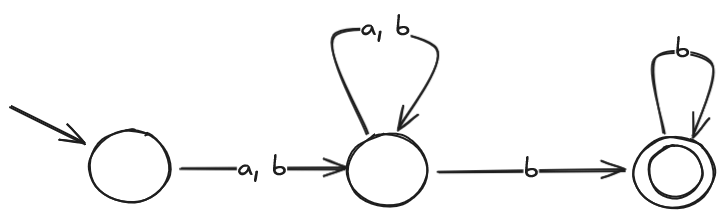
\includegraphics[width=\textwidth]{04-10-02.png}
		\caption{$(b + a)^+b^\omega$}
	\end{subfigure}
	\hfil
	\begin{subfigure}[b]{0.3\textwidth}
		\centering
		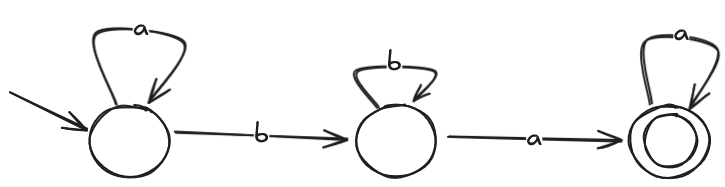
\includegraphics[width=\textwidth]{04-10-03.png}
		\caption{$a^*b^+a^\omega$}
	\end{subfigure}
	\hfil
	\begin{subfigure}[b]{0.3\textwidth}
		\centering
		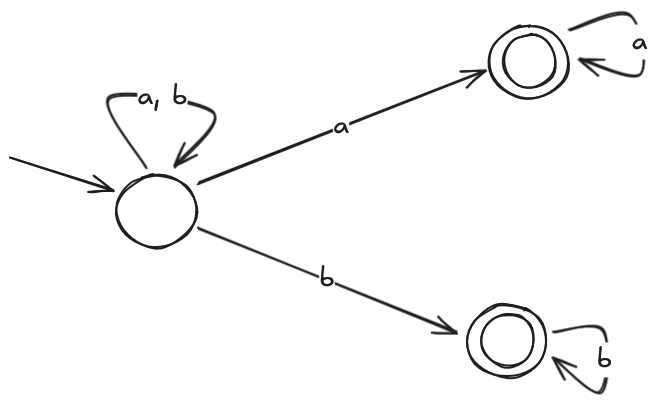
\includegraphics[width=\textwidth]{04-10-04.png}
		\caption{$(a + b)^*(a^\omega + b^\omega)$}
	\end{subfigure}
	\hfil
	\begin{subfigure}[b]{0.3\textwidth}
		\centering
		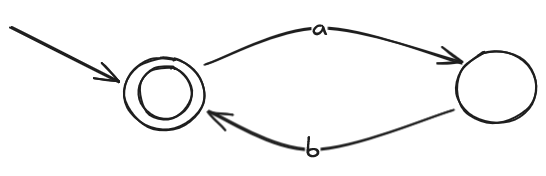
\includegraphics[width=\textwidth]{04-10-05.png}
		\caption{$(ab)^\omega$}
	\end{subfigure}
	\hfil
	\begin{subfigure}[b]{0.2\textwidth}
		\centering
		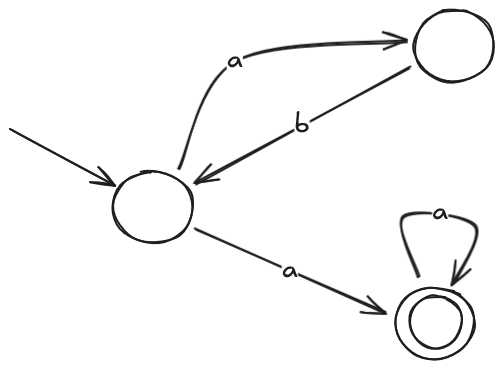
\includegraphics[width=\textwidth]{04-10-06.png}
		\caption{$(ab)^*a^\omega$}
	\end{subfigure}
	\hfil
	\begin{subfigure}[b]{0.3\textwidth}
		\centering
		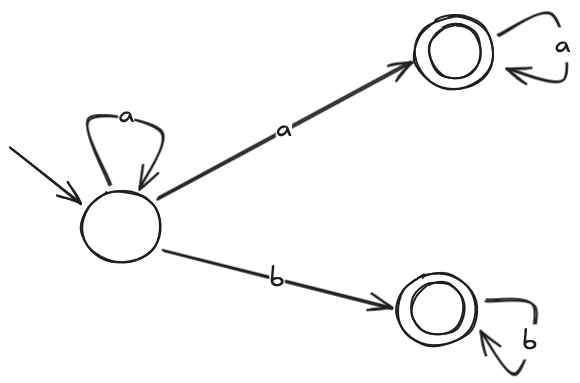
\includegraphics[width=\textwidth]{04-10-07.png}
		\caption{$a^*(a^\omega + b^\omega)$}
	\end{subfigure}
	\hfil
	\begin{subfigure}[b]{0.1\textwidth}
		\centering
		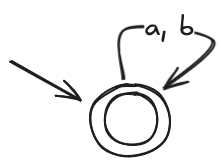
\includegraphics[width=\textwidth]{04-10-08.png}
		\caption{$\Sigma^\omega$}
	\end{subfigure}
	\hfil
	\begin{subfigure}[b]{0.5\textwidth}
		\centering
		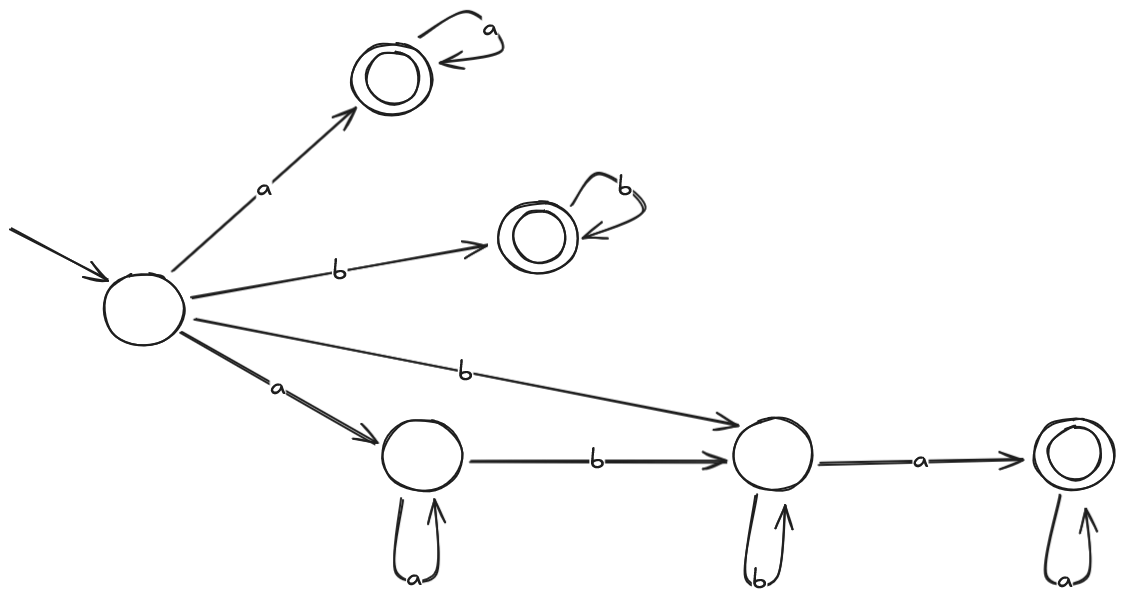
\includegraphics[width=\textwidth]{04-10-09.png}
		\caption{$a^*b^+a^\omega + a^\omega + b^\omega$}
	\end{subfigure}
	\hfil
	\begin{subfigure}[b]{0.3\textwidth}
		\centering
		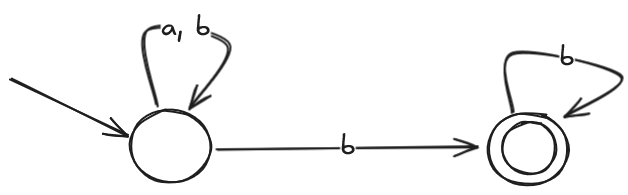
\includegraphics[width=\textwidth]{04-10-10.png}
		\caption{$(a^*b^\omega) + (a + b)^*b^\omega = (a + b)^*b^\omega$}
	\end{subfigure}
	\hfil
	\begin{subfigure}[b]{0.5\textwidth}
		\centering
		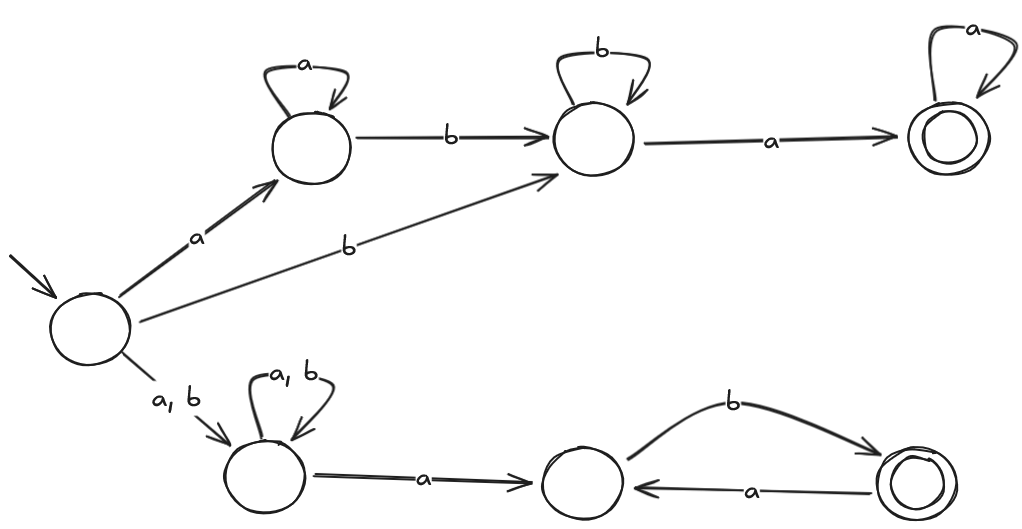
\includegraphics[width=\textwidth]{04-10-11.png}
		\caption{$a^*b^+a^\omega + (a + b)^*(ab)^\omega$}
	\end{subfigure}
	\hfil
	\begin{subfigure}[b]{0.4\textwidth}
		\centering
		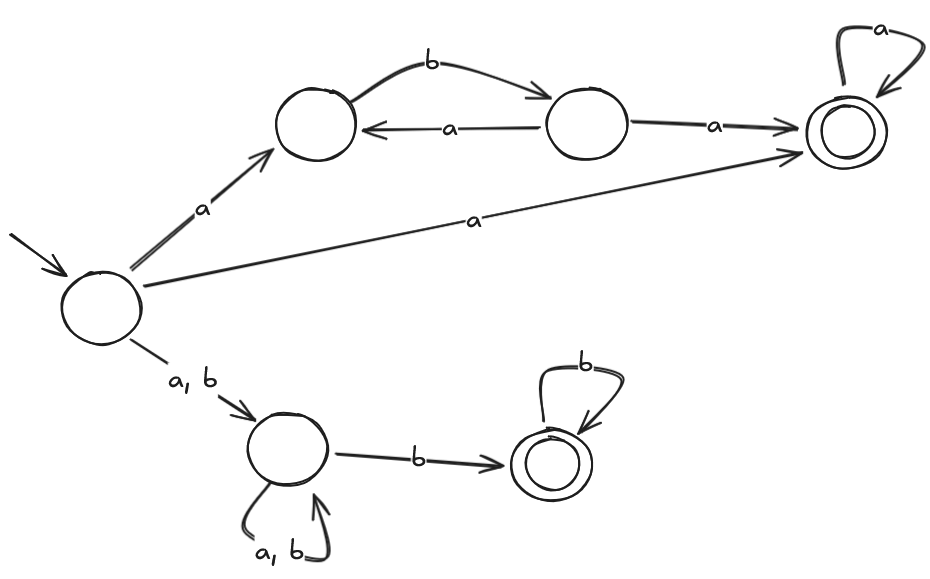
\includegraphics[width=\textwidth]{04-10-12.png}
		\caption{$(ab)^*a^\omega + (a + b)^*b^\omega$}
	\end{subfigure}
\end{figure}

\end{document}
